\section{Vergleichsrechnung mit Newton-Euler-Verfahren}

Die Rechnung wird für debugging-Ziele und eine leichtere Simulation (weniger Rechenintensiv) nur nach der Simulation durchgeführt. 
Deswegen sollen die Daten aus der Simulation in den MATLAB-Workspace übertragen werden. 
Für diese Zwecke kann der \en{ToWorkscape} MATLAB-Block verwendet werden, welcher in Abbildung \ref{fig:simulink_to_workspace} dargestellt ist.
Die Daten in dieser Arbeit werden für jeden Zeitpunkt der Simulation gespeichert.

\begin{figure}[!htbp]
	\centering
	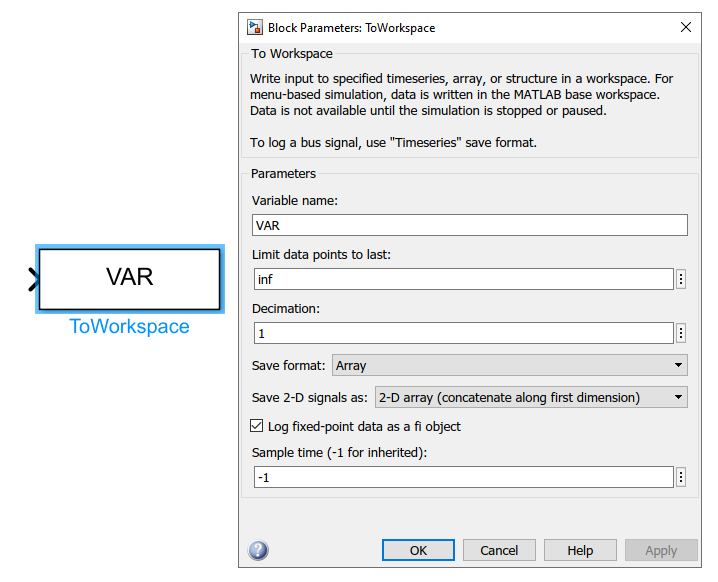
\includegraphics[width=0.59\linewidth]{grafic/to_workspace_block}
	\caption{\en{ToWorkspace}-Block von Matlab}
	\label{fig:simulink_to_workspace}
\end{figure}


\subsection{Abschätzung von Massen und Trägheiten. Ermittlung von Rotationsmatzen, p- und s-Vektoren}

Für die Schätzung der Massen, Trägheiten und s-Vektoren aus der Simulation, steht in Simulink  der \en{Inertia Sensor} zur Verfügung.
Für die Rotationsmatrizen sowie p-Vektoren wird ein \en{Transformation Sensor} verwendet.
Die Sensoren werden in einem Subsystem eingeschlossen. 
Der linke Port des Subsystems entspricht dem Koordinatensystem i, der rechte Port dem Koordinatensystem i+1.
Das Innere des Subsystems ist in der nachfolgenden Abbildung \ref{fig:sensoren_subsystem} zu sehen.

\begin{figure}[!htbp]
	\centering
	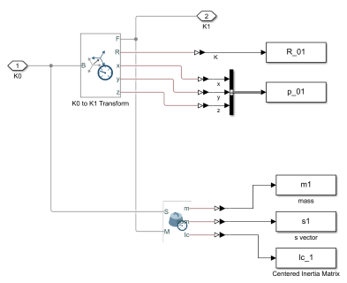
\includegraphics[width=0.54\linewidth]{grafic/sensor_koordinatensystem}
	\caption{Beispiel des Sensorensubsystems}
	\label{fig:sensoren_subsystem}
\end{figure}


\subsection{Berechnung mit Newton-Euler-Verfahren}


\subsubsection{\en{compute\_torques\_with\_newton-euler.m}}

Dieses Skript wird nach der Simulation ausgeführt (StopFnc-Callback in Simulink).
Es führt manche Manipulationen mit den Daten durch, damit sie leichter zu verarbeiten sind.

\begin{lstlisting}[frame=single, basicstyle=\footnotesize, language=Matlab]
if size(q,1) > size(q,2)
q = q';
q_dot = q_dot';
q_2dot = q_2dot';
tau_sim = tau_sim';
end

sim_steps = length(q(1,:));
n_joints = length(q(:,1));

omega = zeros(3, n_joints, sim_steps);
omega_dot = zeros(3, n_joints, sim_steps);
v_dot = zeros(3, n_joints, sim_steps);
vs_dot = zeros(3, n_joints, sim_steps);
tau = zeros(n_joints, sim_steps);

% concatenate data from simulation for easier iteration
R = cat(4, R_01, R_12, R_23, R_34, R_45, R_56);
p = cat(3, p_01', p_12', p_23', p_34', p_45', p_56');
s = cat(3, s1', s2', s3', s4', s5', s6');
Ic = cat(4, Ic_1, Ic_2, Ic_3, Ic_4, Ic_5, Ic_6);
m = cat(1, m1, m2, m3, m4, m5, m6);
m = m';

for i = 1:sim_steps
[omega(:,:,i), omega_dot(:,:,i), v_dot(:,:,i), vs_dot(:,:,i)] = ...
compute_kinematics(q(:,i), q_dot(:,i), q_2dot(:,i), R(:,:,i,:), ...
	R_W0(:,:,i), p(:,i,:), s(:,i,:));
tau(:,i) = compute_forces_and_torques(omega(:,:,i), omega_dot(:,:,i), ...
	vs_dot(:,:,i), m, Ic(:,:,i,:), p(:,i,:), s(:,i,:), R(:,:,i,:));
end

ts = timeseries(tau, tout, 'Name', 'tau');
\end{lstlisting}


\subsubsection{\en{function compute\_kinematics()}}

Die Funktion in Abbildung \ref{fig:sensoren_subsystem_VL} repräsentiert die ersten Schritte des Newton-Euler-Verfahren - \en{kinematische Berechnung}.

\begin{figure}[!htbp]
	\centering
	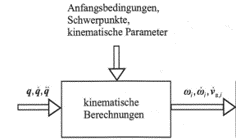
\includegraphics[width=0.42\linewidth]{grafic/compute_kinematics_diagramm}
	\caption{Beispiel des Sensorensubsystems, Quelle: Roboterdynamik, VL 11}
	\label{fig:sensoren_subsystem_VL}
\end{figure}


Die Funktion berechnet die Werte der Geschwindigkeit und Beschleunigungen für K1 mit folgenden Anfangsbedingungen:

\begin{quote}
	$\omega_0 = 0; \hspace{0.5cm} \dot{\omega}_0 = 0; \hspace{0.5cm} \nu = 0; \hspace{0.5cm} \dot{\nu}_0 = -g $
\end{quote}

%\begin{figure}[!htbp]
%	\centering
%	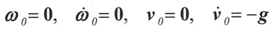
\includegraphics[width=1\linewidth]{grafic/anfangsbedingungen}
%	\caption{Anfangsbedingungen kinematischer Berechnung, Quelle: Roboterdynamik, Vorlesung 11, HHN}
%	\label{fig:anfangsbedingungen}
%\end{figure}


Danach berechnet sie die Werte der Geschwindigkeiten und Beschleunigungen von K2 bis K6 iterativ.

\begin{lstlisting}[frame=single, basicstyle=\footnotesize, language=Matlab]
function [omega, omega_dot, v_dot, vs_dot] = compute_kinematics(q, q_dot, q_2dot, R, R_W0, p, s)
z = [0 0 1]';
n_joints = length(q);

%Anfangsbedingungen
omega = zeros(3, 6);
omega(:,1) = q_dot(1)*z;

omega_dot = zeros(3, 6);
omega_dot(:,1) = q_2dot(1)*z;


% Beschluenigung des KSs.
v_dot(:,1) = inv(R(:,:,1,1)) * (inv(R_W0) * [0 -9.81 0]') + ...
cross(omega_dot(:, 1), p(:,1,1)) + ...
cross(omega(:,1), cross(omega(:,1), p(:,1,1))); 

% Beschleunigung des Schwerpunkts.	
vs_dot(:,1) = v_dot(:,1) + cross(omega_dot(:, 1), s(:, 1, 1)) + ...
cross(omega(:, 1), cross(omega(:,1), s(:, 1, 1))); 

for i = 1:n_joints-1
invR = inv(R(:,:,1,i));

omega(:,i+1) = invR * (omega(:,i) + q_dot(i+1)*z);
omega_dot(:,i+1) = invR * (omega_dot(:,i) + ...
(z * q_2dot(i+1) + cross(omega(:,i), q_dot(i+1) * z)));

v_dot(:, i+1) = invR * v_dot(:,i) + ...
cross(omega_dot(:, i+1), p(:,1,i+1)) + ...
cross(omega(:,i+1), cross(omega(:,i+1), p(:,1,i+1)));
vs_dot(:,i+1) = v_dot(:,i+1) + ...
cross(omega_dot(:, i+1), s(:, 1, i+1)) + ...
cross(omega(:, i+1), cross(omega(:,i+1), s(:, 1, i+1)));
end
end
\end{lstlisting}


Folgende Gleichungen werden in der Funktion verwendet (aus Roboterdynamik, VL 11):

%\begin{quote}
%$\omega_{i+1} = _{i+1}^{i}A$
%\end{quote}
Winkelgeschwindigkeit: 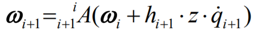
\includegraphics[width=0.4\linewidth]{grafic/omega_gleichung} 

Winkelbeschleunigung: 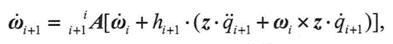
\includegraphics[width=0.6\linewidth]{grafic/omega_dot_gleichung} 

Geschwindigkeit des KSs: 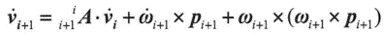
\includegraphics[width=0.64\linewidth]{grafic/v_dot_gleichung}

Geschwindigkeit des Schwerpunkts: 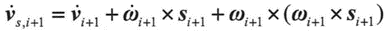
\includegraphics[width=0.63\linewidth]{grafic/vs_dot_gleichung}

%\begin{figure}[!htbp]
%	\centering
%	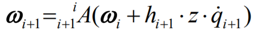
\includegraphics[width=0.5\linewidth]{grafic/omega_gleichung}
%	\caption*{Winkelgeschwindigkeit Gleichung, Quelle: Roboterdynamik, Vorlesung 11, HHN}
%	\label{fig:omega_gleichung}
%\end{figure}
%\begin{figure}[!htbp]
%	\centering
%	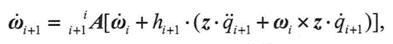
\includegraphics[width=1\linewidth]{grafic/omega_dot_gleichung}
%	\caption{Winkelbeschleunigung Gleichung, Quelle: Roboterdynamik, Vorlesung 11, HHN}
%	\label{fig:omega_dot_gleichung}
%\end{figure}
%\begin{figure}[!htbp]
%	\centering
%	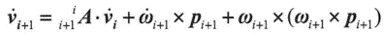
\includegraphics[width=1\linewidth]{grafic/v_dot_gleichung}
%	\caption{Geschwindigkeit des KSs Gleichung, Quelle: Roboterdynamik, Vorlesung 11, HHN}
%	\label{fig:v_dot_gleichung}
%\end{figure}
%\begin{figure}[!htbp]
%	\centering
%	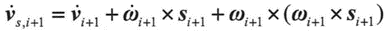
\includegraphics[width=1\linewidth]{grafic/vs_dot_gleichung}
%	\caption{Geschwindigkeit des Schwerpunkts Gleichung, Quelle: Roboterdynamik, Vorlesung 11, HHN}
%	\label{fig:vs_dot_gleichung}
%\end{figure}


\subsubsection{\en{function compute\_forces\_and\_torques()}}

Die Funktion in Abbildung \ref{fig:sensoren_subsystem_foo} repräsentiert den zweiten Schritt des Newton-Euler-Verfahren - \en{Berechnungen der Kräfte und Drehmomente}.

\begin{figure}[!htbp]
	\centering
	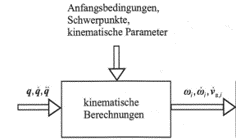
\includegraphics[width=0.43\linewidth]{grafic/compute_kinematics_diagramm}
	\caption{Berechnungen der Kräfte und Drehmomente, Quelle: Roboterdynamik, VL 11}
	\label{fig:sensoren_subsystem_foo}
\end{figure}


\begin{lstlisting}[frame=single, basicstyle=\footnotesize, language=Matlab]
function [tau] = compute_forces_and_torques(omega, omega_dot, vs_dot, m, Ic, p, s, R)
z = [0 0 1]';
n_joints = length(omega(1,:));

% auf n_joints+1 stehen Anfangskraefte- und Drehmomente

f = zeros(3, n_joints+1);
n = zeros(3, n_joints+1);
tau = zeros(1, n_joints);
R(:,:,1,7) = eye(3,3);

for i = n_joints:-1:1
F(:,i) = m(i) * vs_dot(:, i);
f(:,i) = R(:,:,1,i+1) * f(:,i+1) + F(:,i);
N(:,i) = Ic(:,:,1,i) * omega_dot(:,i) + cross(omega(:,i), Ic(:,:,1,i) * omega(:,i));
n(:,i) = n(:,i+1) + cross(p(:,1,i)+s(:,i), F(:,i)) + cross(p(:,i), f(:,i+1)) + N(:,i);
tau(i) = n(:,i)' * inv(R(:,:,1,i)) * z;
end

end
\end{lstlisting}

Folgende Gleichungen werden in der Funktion verwendet (aus Roboterdynamik, VL 11):

%\begin{quote}
%	Kraft an einem Schwerpunkt: $F_{i} = m_i \cdot \dot{\nu}_{s,i}$ 
%\end{quote}

Kraft an einem Schwerpunkt: \; 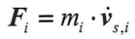
\includegraphics[width=0.15\linewidth]{grafic/Fi_gleichung} 

Gelenkkraft: \; 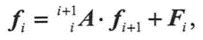
\includegraphics[width=0.28\linewidth]{grafic/klein_fi_gleichung} 

Wirkendendes Drehmoment: 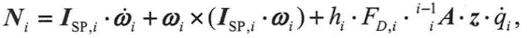
\includegraphics[width=0.62\linewidth]{grafic/gross_n_gleichung} 

Drehmomente im Gelenk: 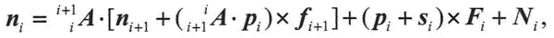
\includegraphics[width=0.68\linewidth]{grafic/klein_n_gleichung} 

Drehmomente im Gelenk: 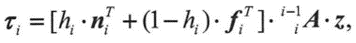
\includegraphics[width=0.5\linewidth]{grafic/tau_gleichung} 

%\begin{figure}[!htbp]
%	\centering
%	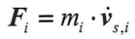
\includegraphics[width=0.15\linewidth]{grafic/Fi_gleichung}
%	\caption*{Kraft an einem Schwerpunkt Gleichung}
%	\label{fig:Fi_gleichung}
%\end{figure}
%\begin{figure}[!htbp]
%	\centering
%	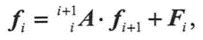
\includegraphics[width=0.28\linewidth]{grafic/klein_fi_gleichung}
%	\caption*{Gelenkkraft Gleichung}
%	\label{fig:klein_fi_gleichung}
%\end{figure}
%\begin{figure}[!htbp]
%	\centering
%	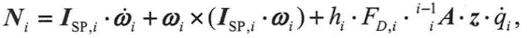
\includegraphics[width=0.55\linewidth]{grafic/gross_n_gleichung}
%	\caption*{Wirkenden Drehmonent Gleichung}
%	\label{fig:gross_n_gleichung}
%\\\end{figure}
%\begin{figure}[!htbp]
%	\centering
%	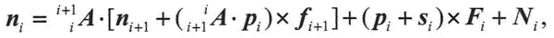
\includegraphics[width=0.6\linewidth]{grafic/klein_n_gleichung}
%	\caption*{Drehmomente in dem Gelenk Gleichung}
%	\label{fig:klein_n_gleichung}
%\end{figure}
%\begin{figure}[!htbp]
%	\centering
%	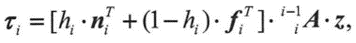
\includegraphics[width=1\linewidth]{grafic/tau_gleichung}
%	\caption{Drehmomente in dem Gelenk Gleichung, Quelle: Roboterdynamik, Vorlesung 11, HHN}
%	\label{fig:tau_gleichung}
%\end{figure}





